% Options for packages loaded elsewhere
% Options for packages loaded elsewhere
\PassOptionsToPackage{unicode}{hyperref}
\PassOptionsToPackage{hyphens}{url}
\PassOptionsToPackage{dvipsnames,svgnames,x11names}{xcolor}
%
\documentclass[
  letterpaper,
  DIV=11,
  numbers=noendperiod]{scrartcl}
\usepackage{xcolor}
\usepackage{amsmath,amssymb}
\setcounter{secnumdepth}{-\maxdimen} % remove section numbering
\usepackage{iftex}
\ifPDFTeX
  \usepackage[T1]{fontenc}
  \usepackage[utf8]{inputenc}
  \usepackage{textcomp} % provide euro and other symbols
\else % if luatex or xetex
  \usepackage{unicode-math} % this also loads fontspec
  \defaultfontfeatures{Scale=MatchLowercase}
  \defaultfontfeatures[\rmfamily]{Ligatures=TeX,Scale=1}
\fi
\usepackage{lmodern}
\ifPDFTeX\else
  % xetex/luatex font selection
\fi
% Use upquote if available, for straight quotes in verbatim environments
\IfFileExists{upquote.sty}{\usepackage{upquote}}{}
\IfFileExists{microtype.sty}{% use microtype if available
  \usepackage[]{microtype}
  \UseMicrotypeSet[protrusion]{basicmath} % disable protrusion for tt fonts
}{}
\makeatletter
\@ifundefined{KOMAClassName}{% if non-KOMA class
  \IfFileExists{parskip.sty}{%
    \usepackage{parskip}
  }{% else
    \setlength{\parindent}{0pt}
    \setlength{\parskip}{6pt plus 2pt minus 1pt}}
}{% if KOMA class
  \KOMAoptions{parskip=half}}
\makeatother
% Make \paragraph and \subparagraph free-standing
\makeatletter
\ifx\paragraph\undefined\else
  \let\oldparagraph\paragraph
  \renewcommand{\paragraph}{
    \@ifstar
      \xxxParagraphStar
      \xxxParagraphNoStar
  }
  \newcommand{\xxxParagraphStar}[1]{\oldparagraph*{#1}\mbox{}}
  \newcommand{\xxxParagraphNoStar}[1]{\oldparagraph{#1}\mbox{}}
\fi
\ifx\subparagraph\undefined\else
  \let\oldsubparagraph\subparagraph
  \renewcommand{\subparagraph}{
    \@ifstar
      \xxxSubParagraphStar
      \xxxSubParagraphNoStar
  }
  \newcommand{\xxxSubParagraphStar}[1]{\oldsubparagraph*{#1}\mbox{}}
  \newcommand{\xxxSubParagraphNoStar}[1]{\oldsubparagraph{#1}\mbox{}}
\fi
\makeatother

\usepackage{color}
\usepackage{fancyvrb}
\newcommand{\VerbBar}{|}
\newcommand{\VERB}{\Verb[commandchars=\\\{\}]}
\DefineVerbatimEnvironment{Highlighting}{Verbatim}{commandchars=\\\{\}}
% Add ',fontsize=\small' for more characters per line
\usepackage{framed}
\definecolor{shadecolor}{RGB}{241,243,245}
\newenvironment{Shaded}{\begin{snugshade}}{\end{snugshade}}
\newcommand{\AlertTok}[1]{\textcolor[rgb]{0.68,0.00,0.00}{#1}}
\newcommand{\AnnotationTok}[1]{\textcolor[rgb]{0.37,0.37,0.37}{#1}}
\newcommand{\AttributeTok}[1]{\textcolor[rgb]{0.40,0.45,0.13}{#1}}
\newcommand{\BaseNTok}[1]{\textcolor[rgb]{0.68,0.00,0.00}{#1}}
\newcommand{\BuiltInTok}[1]{\textcolor[rgb]{0.00,0.23,0.31}{#1}}
\newcommand{\CharTok}[1]{\textcolor[rgb]{0.13,0.47,0.30}{#1}}
\newcommand{\CommentTok}[1]{\textcolor[rgb]{0.37,0.37,0.37}{#1}}
\newcommand{\CommentVarTok}[1]{\textcolor[rgb]{0.37,0.37,0.37}{\textit{#1}}}
\newcommand{\ConstantTok}[1]{\textcolor[rgb]{0.56,0.35,0.01}{#1}}
\newcommand{\ControlFlowTok}[1]{\textcolor[rgb]{0.00,0.23,0.31}{\textbf{#1}}}
\newcommand{\DataTypeTok}[1]{\textcolor[rgb]{0.68,0.00,0.00}{#1}}
\newcommand{\DecValTok}[1]{\textcolor[rgb]{0.68,0.00,0.00}{#1}}
\newcommand{\DocumentationTok}[1]{\textcolor[rgb]{0.37,0.37,0.37}{\textit{#1}}}
\newcommand{\ErrorTok}[1]{\textcolor[rgb]{0.68,0.00,0.00}{#1}}
\newcommand{\ExtensionTok}[1]{\textcolor[rgb]{0.00,0.23,0.31}{#1}}
\newcommand{\FloatTok}[1]{\textcolor[rgb]{0.68,0.00,0.00}{#1}}
\newcommand{\FunctionTok}[1]{\textcolor[rgb]{0.28,0.35,0.67}{#1}}
\newcommand{\ImportTok}[1]{\textcolor[rgb]{0.00,0.46,0.62}{#1}}
\newcommand{\InformationTok}[1]{\textcolor[rgb]{0.37,0.37,0.37}{#1}}
\newcommand{\KeywordTok}[1]{\textcolor[rgb]{0.00,0.23,0.31}{\textbf{#1}}}
\newcommand{\NormalTok}[1]{\textcolor[rgb]{0.00,0.23,0.31}{#1}}
\newcommand{\OperatorTok}[1]{\textcolor[rgb]{0.37,0.37,0.37}{#1}}
\newcommand{\OtherTok}[1]{\textcolor[rgb]{0.00,0.23,0.31}{#1}}
\newcommand{\PreprocessorTok}[1]{\textcolor[rgb]{0.68,0.00,0.00}{#1}}
\newcommand{\RegionMarkerTok}[1]{\textcolor[rgb]{0.00,0.23,0.31}{#1}}
\newcommand{\SpecialCharTok}[1]{\textcolor[rgb]{0.37,0.37,0.37}{#1}}
\newcommand{\SpecialStringTok}[1]{\textcolor[rgb]{0.13,0.47,0.30}{#1}}
\newcommand{\StringTok}[1]{\textcolor[rgb]{0.13,0.47,0.30}{#1}}
\newcommand{\VariableTok}[1]{\textcolor[rgb]{0.07,0.07,0.07}{#1}}
\newcommand{\VerbatimStringTok}[1]{\textcolor[rgb]{0.13,0.47,0.30}{#1}}
\newcommand{\WarningTok}[1]{\textcolor[rgb]{0.37,0.37,0.37}{\textit{#1}}}

\usepackage{longtable,booktabs,array}
\newcounter{none} % for unnumbered tables
\usepackage{calc} % for calculating minipage widths
% Correct order of tables after \paragraph or \subparagraph
\usepackage{etoolbox}
\makeatletter
\patchcmd\longtable{\par}{\if@noskipsec\mbox{}\fi\par}{}{}
\makeatother
% Allow footnotes in longtable head/foot
\IfFileExists{footnotehyper.sty}{\usepackage{footnotehyper}}{\usepackage{footnote}}
\makesavenoteenv{longtable}
\usepackage{graphicx}
\makeatletter
\newsavebox\pandoc@box
\newcommand*\pandocbounded[1]{% scales image to fit in text height/width
  \sbox\pandoc@box{#1}%
  \Gscale@div\@tempa{\textheight}{\dimexpr\ht\pandoc@box+\dp\pandoc@box\relax}%
  \Gscale@div\@tempb{\linewidth}{\wd\pandoc@box}%
  \ifdim\@tempb\p@<\@tempa\p@\let\@tempa\@tempb\fi% select the smaller of both
  \ifdim\@tempa\p@<\p@\scalebox{\@tempa}{\usebox\pandoc@box}%
  \else\usebox{\pandoc@box}%
  \fi%
}
% Set default figure placement to htbp
\def\fps@figure{htbp}
\makeatother





\setlength{\emergencystretch}{3em} % prevent overfull lines

\providecommand{\tightlist}{%
  \setlength{\itemsep}{0pt}\setlength{\parskip}{0pt}}



 


\KOMAoption{captions}{tableheading}
\makeatletter
\@ifpackageloaded{caption}{}{\usepackage{caption}}
\AtBeginDocument{%
\ifdefined\contentsname
  \renewcommand*\contentsname{Table of contents}
\else
  \newcommand\contentsname{Table of contents}
\fi
\ifdefined\listfigurename
  \renewcommand*\listfigurename{List of Figures}
\else
  \newcommand\listfigurename{List of Figures}
\fi
\ifdefined\listtablename
  \renewcommand*\listtablename{List of Tables}
\else
  \newcommand\listtablename{List of Tables}
\fi
\ifdefined\figurename
  \renewcommand*\figurename{Figure}
\else
  \newcommand\figurename{Figure}
\fi
\ifdefined\tablename
  \renewcommand*\tablename{Table}
\else
  \newcommand\tablename{Table}
\fi
}
\@ifpackageloaded{float}{}{\usepackage{float}}
\floatstyle{ruled}
\@ifundefined{c@chapter}{\newfloat{codelisting}{h}{lop}}{\newfloat{codelisting}{h}{lop}[chapter]}
\floatname{codelisting}{Listing}
\newcommand*\listoflistings{\listof{codelisting}{List of Listings}}
\makeatother
\makeatletter
\makeatother
\makeatletter
\@ifpackageloaded{caption}{}{\usepackage{caption}}
\@ifpackageloaded{subcaption}{}{\usepackage{subcaption}}
\makeatother
\usepackage{bookmark}
\IfFileExists{xurl.sty}{\usepackage{xurl}}{} % add URL line breaks if available
\urlstyle{same}
\hypersetup{
  colorlinks=true,
  linkcolor={blue},
  filecolor={Maroon},
  citecolor={Blue},
  urlcolor={Blue},
  pdfcreator={LaTeX via pandoc}}


\author{}
\date{}
\begin{document}


\begin{Shaded}
\begin{Highlighting}[]
\CommentTok{\# Instalação de pacotes necessários}
\NormalTok{pkgs }\OtherTok{\textless{}{-}} \FunctionTok{c}\NormalTok{(}
  \StringTok{"tidymodels"}\NormalTok{,}
  \StringTok{\textquotesingle{}glmnet\textquotesingle{}}\NormalTok{,}
  \StringTok{"rstanarm"}
\NormalTok{)}

\NormalTok{instalar }\OtherTok{\textless{}{-}}\NormalTok{ pkgs[}\SpecialCharTok{!}\NormalTok{pkgs }\SpecialCharTok{\%in\%} \FunctionTok{installed.packages}\NormalTok{()[, }\StringTok{"Package"}\NormalTok{]]}

\ControlFlowTok{if}\NormalTok{ (}\FunctionTok{length}\NormalTok{(instalar) }\SpecialCharTok{\textgreater{}} \DecValTok{0}\NormalTok{) \{}
  \FunctionTok{install.packages}\NormalTok{(instalar)}
\NormalTok{\}}
\end{Highlighting}
\end{Shaded}

\begin{Shaded}
\begin{Highlighting}[]
\FunctionTok{library}\NormalTok{(tidyverse)}
\FunctionTok{library}\NormalTok{(}\StringTok{"tidymodels"}\NormalTok{)}
\FunctionTok{library}\NormalTok{(}\StringTok{\textquotesingle{}janitor\textquotesingle{}}\NormalTok{)}
\FunctionTok{library}\NormalTok{(}\StringTok{\textquotesingle{}ggcorrplot\textquotesingle{}}\NormalTok{)}
\FunctionTok{library}\NormalTok{(workflowsets)}
\FunctionTok{library}\NormalTok{(rstanarm)}
\FunctionTok{library}\NormalTok{(glmnet)}
\end{Highlighting}
\end{Shaded}

\begin{Shaded}
\begin{Highlighting}[]
\CommentTok{\#}
\FunctionTok{set.seed}\NormalTok{(}\DecValTok{42}\NormalTok{)}
\end{Highlighting}
\end{Shaded}

\begin{Shaded}
\begin{Highlighting}[]
\NormalTok{loan }\OtherTok{\textless{}{-}} \FunctionTok{read\_csv}\NormalTok{(}\StringTok{"../data/Loan/loan\_approval\_dataset.csv"}\NormalTok{) }\SpecialCharTok{|\textgreater{}}
  \FunctionTok{clean\_names}\NormalTok{()}
\end{Highlighting}
\end{Shaded}

\begin{verbatim}
Rows: 4269 Columns: 13
── Column specification ────────────────────────────────────────────────────────
Delimiter: ","
chr  (3): education, self_employed, loan_status
dbl (10): loan_id, no_of_dependents, income_annum, loan_amount, loan_term, c...

ℹ Use `spec()` to retrieve the full column specification for this data.
ℹ Specify the column types or set `show_col_types = FALSE` to quiet this message.
\end{verbatim}

\begin{Shaded}
\begin{Highlighting}[]
\CommentTok{\#preprocessamento}
\NormalTok{loan }\OtherTok{\textless{}{-}}\NormalTok{ janitor}\SpecialCharTok{::}\FunctionTok{clean\_names}\NormalTok{(loan)}

\NormalTok{loan }\OtherTok{\textless{}{-}}\NormalTok{ loan }\SpecialCharTok{|\textgreater{}}
\NormalTok{  dplyr}\SpecialCharTok{::}\FunctionTok{filter}\NormalTok{(residential\_assets\_value }\SpecialCharTok{\textgreater{}=} \DecValTok{0}\NormalTok{)}
\end{Highlighting}
\end{Shaded}

\begin{Shaded}
\begin{Highlighting}[]
\NormalTok{loan\_num }\OtherTok{\textless{}{-}}\NormalTok{ loan }\SpecialCharTok{|\textgreater{}}
\NormalTok{  dplyr}\SpecialCharTok{::}\FunctionTok{select}\NormalTok{(}\FunctionTok{where}\NormalTok{(is.numeric))}

\NormalTok{cor\_matrix }\OtherTok{\textless{}{-}} \FunctionTok{cor}\NormalTok{(}
\NormalTok{  loan\_num,}
  \AttributeTok{use =} \StringTok{"complete.obs"}\NormalTok{,}
  \AttributeTok{method =} \StringTok{"pearson"}
\NormalTok{)}

\FunctionTok{ggcorrplot}\NormalTok{(}
\NormalTok{  cor\_matrix,}
  \AttributeTok{type =} \StringTok{"lower"}\NormalTok{,}
  \AttributeTok{lab =} \ConstantTok{TRUE}\NormalTok{,}
  \AttributeTok{lab\_size =} \DecValTok{4}\NormalTok{,}
  \AttributeTok{colors =} \FunctionTok{c}\NormalTok{(}\StringTok{"\#b2182b"}\NormalTok{, }\StringTok{"white"}\NormalTok{, }\StringTok{"\#2166ac"}\NormalTok{),}
  \AttributeTok{outline.col =} \StringTok{"gray70"}
\NormalTok{) }\SpecialCharTok{+}
  \FunctionTok{theme\_minimal}\NormalTok{(}\AttributeTok{base\_size =} \DecValTok{14}\NormalTok{) }\SpecialCharTok{+}
  \FunctionTok{theme}\NormalTok{(}
    \AttributeTok{axis.text.x =} \FunctionTok{element\_text}\NormalTok{(}
      \AttributeTok{angle =} \DecValTok{90}\NormalTok{,}
      \AttributeTok{hjust =} \DecValTok{1}\NormalTok{,}
      \AttributeTok{vjust =} \FloatTok{0.5}
\NormalTok{    ),}
    \AttributeTok{axis.text.y =} \FunctionTok{element\_text}\NormalTok{(}\AttributeTok{size =} \DecValTok{8}\NormalTok{)}
\NormalTok{  )}
\end{Highlighting}
\end{Shaded}

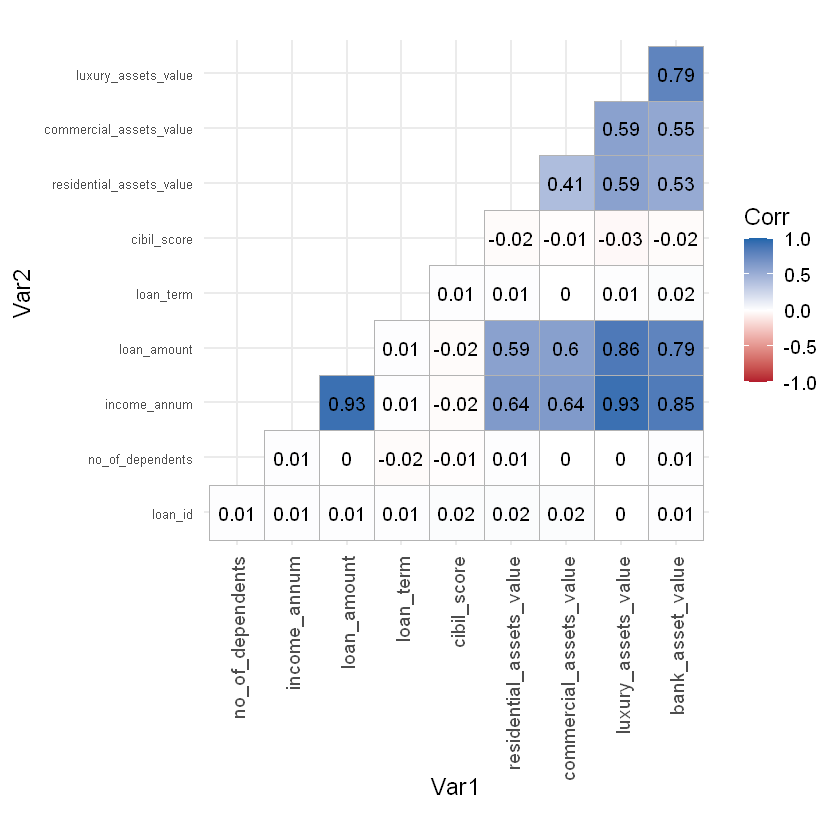
\includegraphics[width=4.375in,height=4.375in]{modeling_notencoded_files/figure-pdf/cell-7-output-1.png}

\begin{Shaded}
\begin{Highlighting}[]
\NormalTok{vars\_categoricas }\OtherTok{\textless{}{-}} \FunctionTok{c}\NormalTok{(}
  \StringTok{"education"}\NormalTok{,}
  \StringTok{"self\_employed"}
\NormalTok{)}

\NormalTok{vars\_numericas }\OtherTok{\textless{}{-}} \FunctionTok{c}\NormalTok{(}
  \StringTok{"no\_of\_dependents"}\NormalTok{,}
  \StringTok{"income\_annum"}\NormalTok{,}
  \StringTok{"loan\_amount"}\NormalTok{,}
  \StringTok{"loan\_term"}\NormalTok{,}
  \StringTok{"cibil\_score"}\NormalTok{,}
  \StringTok{"residential\_assets\_value"}\NormalTok{,}
  \StringTok{"commercial\_assets\_value"}\NormalTok{,}
  \StringTok{"luxury\_assets\_value"}\NormalTok{,}
  \StringTok{"bank\_asset\_value"}
\NormalTok{)}

\CommentTok{\# One{-}Hot Encoding}
\NormalTok{loan\_encoded }\OtherTok{\textless{}{-}}\NormalTok{ loan }\SpecialCharTok{\%\textgreater{}\%}
  \FunctionTok{mutate}\NormalTok{(}
    \AttributeTok{education =} \FunctionTok{factor}\NormalTok{(education),}
    \AttributeTok{self\_employed =} \FunctionTok{factor}\NormalTok{(self\_employed)}
\NormalTok{  ) }\SpecialCharTok{\%\textgreater{}\%}
\NormalTok{  fastDummies}\SpecialCharTok{::}\FunctionTok{dummy\_cols}\NormalTok{(}
    \AttributeTok{select\_columns =}\NormalTok{ vars\_categoricas,}
    \AttributeTok{remove\_selected\_columns =} \ConstantTok{TRUE}\NormalTok{,}
    \AttributeTok{remove\_first\_dummy =} \ConstantTok{TRUE}
\NormalTok{  )}

\CommentTok{\# Padronização (Standardization)}
\CommentTok{\#loan\_encoded[vars\_numericas] \textless{}{-} lapply(}
\CommentTok{\#  loan\_encoded[vars\_numericas],}
\CommentTok{\#  function(x) as.numeric(as.character(x))}
\CommentTok{\#)}
\CommentTok{\#loan\_encoded[vars\_numericas] \textless{}{-} scale(loan\_encoded[vars\_numericas])}
\end{Highlighting}
\end{Shaded}

\begin{Shaded}
\begin{Highlighting}[]
\CommentTok{\#remodendo loan id}
\NormalTok{loan\_encoded }\OtherTok{\textless{}{-}}\NormalTok{ loan\_encoded }\SpecialCharTok{|\textgreater{}}
\NormalTok{  dplyr}\SpecialCharTok{::}\FunctionTok{select}\NormalTok{(}\SpecialCharTok{{-}}\NormalTok{loan\_id)}

\NormalTok{loan\_encoded}\SpecialCharTok{$}\NormalTok{loan\_status }\OtherTok{\textless{}{-}} \FunctionTok{ifelse}\NormalTok{(}
\NormalTok{  loan\_encoded}\SpecialCharTok{$}\NormalTok{loan\_status }\SpecialCharTok{\%in\%} \FunctionTok{c}\NormalTok{(}\StringTok{"Approved"}\NormalTok{, }\DecValTok{1}\NormalTok{, }\StringTok{"1"}\NormalTok{),}
  \DecValTok{1}\NormalTok{, }\DecValTok{0}
\NormalTok{)}
\NormalTok{loan\_encoded}\SpecialCharTok{$}\NormalTok{loan\_status }\OtherTok{\textless{}{-}} \FunctionTok{as.factor}\NormalTok{(loan\_encoded}\SpecialCharTok{$}\NormalTok{loan\_status)}


\NormalTok{split }\OtherTok{\textless{}{-}} \FunctionTok{initial\_split}\NormalTok{(}
\NormalTok{  loan\_encoded,}
  \AttributeTok{prop   =} \FloatTok{0.75}\NormalTok{,}
  \AttributeTok{strata =}\NormalTok{ loan\_status}
\NormalTok{)}

\NormalTok{train\_data }\OtherTok{\textless{}{-}} \FunctionTok{training}\NormalTok{(split)}
\NormalTok{test\_data  }\OtherTok{\textless{}{-}} \FunctionTok{testing}\NormalTok{(split)}
\end{Highlighting}
\end{Shaded}

\begin{Shaded}
\begin{Highlighting}[]
\CommentTok{\# One{-}Hot Encoding}
\NormalTok{loan\_ohe }\OtherTok{\textless{}{-}}\NormalTok{ loan }\SpecialCharTok{\%\textgreater{}\%}
  \FunctionTok{mutate}\NormalTok{(}
    \AttributeTok{education =} \FunctionTok{factor}\NormalTok{(education),}
    \AttributeTok{self\_employed =} \FunctionTok{factor}\NormalTok{(self\_employed)}
\NormalTok{  ) }\SpecialCharTok{\%\textgreater{}\%}
\NormalTok{  fastDummies}\SpecialCharTok{::}\FunctionTok{dummy\_cols}\NormalTok{(}
    \AttributeTok{select\_columns =}\NormalTok{ vars\_categoricas,}
    \AttributeTok{remove\_selected\_columns =} \ConstantTok{TRUE}\NormalTok{,}
    \AttributeTok{remove\_first\_dummy =} \ConstantTok{TRUE}
\NormalTok{  )}
\NormalTok{split }\OtherTok{\textless{}{-}} \FunctionTok{initial\_split}\NormalTok{(}
\NormalTok{  loan\_ohe,}
  \AttributeTok{prop   =} \FloatTok{0.75}\NormalTok{,}
  \AttributeTok{strata =}\NormalTok{ loan\_status}
\NormalTok{)}

\NormalTok{train\_data\_not }\OtherTok{\textless{}{-}} \FunctionTok{training}\NormalTok{(split)}
\NormalTok{test\_data\_not  }\OtherTok{\textless{}{-}} \FunctionTok{testing}\NormalTok{(split)}
\end{Highlighting}
\end{Shaded}

\begin{Shaded}
\begin{Highlighting}[]
\FunctionTok{count}\NormalTok{(train\_data, loan\_status)}
\FunctionTok{count}\NormalTok{(test\_data, loan\_status)}
\end{Highlighting}
\end{Shaded}

A tibble: 2 × 2

{\def\LTcaptype{none} % do not increment counter
\begin{longtable}[]{@{}ll@{}}
\toprule\noalign{}
loan\_status \textless fct\textgreater{} & n
\textless int\textgreater{} \\
\midrule\noalign{}
\endhead
\bottomrule\noalign{}
\endlastfoot
0 & 1200 \\
1 & 1980 \\
\end{longtable}
}

A tibble: 2 × 2

{\def\LTcaptype{none} % do not increment counter
\begin{longtable}[]{@{}ll@{}}
\toprule\noalign{}
loan\_status \textless fct\textgreater{} & n
\textless int\textgreater{} \\
\midrule\noalign{}
\endhead
\bottomrule\noalign{}
\endlastfoot
0 & 401 \\
1 & 660 \\
\end{longtable}
}

para o frequentista - Modelo geral (tudo) OK - Modelo apenas com score
Ok - Modelo sem score ok - Modelo com remoção das feats correlacionadas
ok - Modelo com PCA - Modelo com regularização para selecionar feats
(glmnet) ok

\begin{Shaded}
\begin{Highlighting}[]
\NormalTok{rec\_lasso }\OtherTok{\textless{}{-}} \FunctionTok{recipe}\NormalTok{(loan\_status }\SpecialCharTok{\textasciitilde{}}\NormalTok{ ., }\AttributeTok{data =}\NormalTok{ train\_data) }\SpecialCharTok{\%\textgreater{}\%}
  \FunctionTok{step\_dummy}\NormalTok{(}\FunctionTok{all\_nominal\_predictors}\NormalTok{()) }\SpecialCharTok{\%\textgreater{}\%}
  \FunctionTok{step\_normalize}\NormalTok{(}\FunctionTok{all\_numeric\_predictors}\NormalTok{())}

\NormalTok{logit\_lasso\_spec }\OtherTok{\textless{}{-}} \FunctionTok{logistic\_reg}\NormalTok{(}
  \AttributeTok{penalty =} \FunctionTok{tune}\NormalTok{(),}
  \AttributeTok{mixture =} \DecValTok{1}        \CommentTok{\# LASSO puro}
\NormalTok{) }\SpecialCharTok{\%\textgreater{}\%}
  \FunctionTok{set\_engine}\NormalTok{(}\StringTok{"glmnet"}\NormalTok{)}

\NormalTok{wf\_lasso }\OtherTok{\textless{}{-}} \FunctionTok{workflow}\NormalTok{() }\SpecialCharTok{\%\textgreater{}\%}
  \FunctionTok{add\_recipe}\NormalTok{(rec\_lasso) }\SpecialCharTok{\%\textgreater{}\%}
  \FunctionTok{add\_model}\NormalTok{(logit\_lasso\_spec)}


\NormalTok{folds }\OtherTok{\textless{}{-}} \FunctionTok{vfold\_cv}\NormalTok{(train\_data, }\AttributeTok{v =} \DecValTok{5}\NormalTok{)}

\NormalTok{grid\_lambda }\OtherTok{\textless{}{-}} \FunctionTok{grid\_regular}\NormalTok{(}\FunctionTok{penalty}\NormalTok{(), }\AttributeTok{levels =} \DecValTok{50}\NormalTok{)}

\NormalTok{lasso\_res }\OtherTok{\textless{}{-}} \FunctionTok{tune\_grid}\NormalTok{(}
\NormalTok{  wf\_lasso,}
  \AttributeTok{resamples =}\NormalTok{ folds,}
  \AttributeTok{grid =}\NormalTok{ grid\_lambda,}
  \AttributeTok{metrics =} \FunctionTok{metric\_set}\NormalTok{(roc\_auc)}
\NormalTok{)  }
\NormalTok{best\_lambda }\OtherTok{\textless{}{-}} \FunctionTok{select\_best}\NormalTok{(lasso\_res, }\AttributeTok{metric =} \StringTok{"roc\_auc"}\NormalTok{)}
\NormalTok{best\_lambda}
\end{Highlighting}
\end{Shaded}

A tibble: 1 × 2

{\def\LTcaptype{none} % do not increment counter
\begin{longtable}[]{@{}ll@{}}
\toprule\noalign{}
penalty \textless dbl\textgreater{} & .config
\textless chr\textgreater{} \\
\midrule\noalign{}
\endhead
\bottomrule\noalign{}
\endlastfoot
0.001389495 & pre0\_mod36\_post0 \\
\end{longtable}
}

\begin{Shaded}
\begin{Highlighting}[]
\NormalTok{final\_lasso\_wf }\OtherTok{\textless{}{-}} \FunctionTok{finalize\_workflow}\NormalTok{(}
\NormalTok{  wf\_lasso,}
\NormalTok{  best\_lambda}
\NormalTok{)}

\NormalTok{final\_lasso\_fit }\OtherTok{\textless{}{-}} \FunctionTok{fit}\NormalTok{(}
\NormalTok{  final\_lasso\_wf,}
  \AttributeTok{data =}\NormalTok{ train\_data}
\NormalTok{)}

\NormalTok{lasso\_coefs }\OtherTok{\textless{}{-}}\NormalTok{ final\_lasso\_fit }\SpecialCharTok{\%\textgreater{}\%}
  \FunctionTok{extract\_fit\_parsnip}\NormalTok{() }\SpecialCharTok{\%\textgreater{}\%}
  \FunctionTok{tidy}\NormalTok{()}

\NormalTok{vars\_selected }\OtherTok{\textless{}{-}}\NormalTok{ lasso\_coefs }\SpecialCharTok{\%\textgreater{}\%}
  \FunctionTok{filter}\NormalTok{(term }\SpecialCharTok{!=} \StringTok{"(Intercept)"}\NormalTok{) }\SpecialCharTok{\%\textgreater{}\%}
  \FunctionTok{filter}\NormalTok{(estimate }\SpecialCharTok{!=} \DecValTok{0}\NormalTok{) }\SpecialCharTok{\%\textgreater{}\%}
  \FunctionTok{mutate}\NormalTok{(}\AttributeTok{abs\_est =} \FunctionTok{abs}\NormalTok{(estimate))}
\NormalTok{vars\_importance }\OtherTok{\textless{}{-}}\NormalTok{ vars\_selected }\SpecialCharTok{\%\textgreater{}\%}
  \FunctionTok{mutate}\NormalTok{(}\AttributeTok{importance =}\NormalTok{ abs\_est }\SpecialCharTok{/} \FunctionTok{sum}\NormalTok{(abs\_est)) }\SpecialCharTok{\%\textgreater{}\%}
  \FunctionTok{select}\NormalTok{(}\AttributeTok{variable =}\NormalTok{ term, importance) }\SpecialCharTok{\%\textgreater{}\%}
  \FunctionTok{arrange}\NormalTok{(}\FunctionTok{desc}\NormalTok{(importance))}

\NormalTok{vars\_importance}
\end{Highlighting}
\end{Shaded}

A tibble: 9 × 2

{\def\LTcaptype{none} % do not increment counter
\begin{longtable}[]{@{}ll@{}}
\toprule\noalign{}
variable \textless chr\textgreater{} & importance
\textless dbl\textgreater{} \\
\midrule\noalign{}
\endhead
\bottomrule\noalign{}
\endlastfoot
cibil\_score & 0.578373789 \\
income\_annum & 0.144973617 \\
loan\_amount & 0.133237908 \\
loan\_term & 0.114876889 \\
bank\_asset\_value & 0.009355327 \\
commercial\_assets\_value & 0.006429094 \\
no\_of\_dependents & 0.006130255 \\
self\_employed\_Yes & 0.004360122 \\
education\_Not Graduate & 0.002262998 \\
\end{longtable}
}

\begin{Shaded}
\begin{Highlighting}[]
\NormalTok{not\_best\_vars }\OtherTok{\textless{}{-}}\NormalTok{ vars\_importance }\SpecialCharTok{\%\textgreater{}\%}
\NormalTok{  dplyr}\SpecialCharTok{::}\FunctionTok{filter}\NormalTok{(importance }\SpecialCharTok{\textless{}} \FloatTok{0.10}\NormalTok{) }\SpecialCharTok{\%\textgreater{}\%}
\NormalTok{  dplyr}\SpecialCharTok{::}\FunctionTok{pull}\NormalTok{(variable)}
\end{Highlighting}
\end{Shaded}

\begin{Shaded}
\begin{Highlighting}[]
\CommentTok{\#modelo geral}
\NormalTok{rec\_all }\OtherTok{\textless{}{-}} \FunctionTok{recipe}\NormalTok{(loan\_status }\SpecialCharTok{\textasciitilde{}}\NormalTok{ ., }\AttributeTok{data =}\NormalTok{ train\_data)}
\NormalTok{rec\_all\_not }\OtherTok{\textless{}{-}} \FunctionTok{recipe}\NormalTok{(loan\_status }\SpecialCharTok{\textasciitilde{}}\NormalTok{ ., }\AttributeTok{data =}\NormalTok{ train\_data\_not)}

\CommentTok{\# score only}
\NormalTok{rec\_score\_only }\OtherTok{\textless{}{-}} \FunctionTok{recipe}\NormalTok{(}
\NormalTok{  loan\_status }\SpecialCharTok{\textasciitilde{}}\NormalTok{ cibil\_score,}
  \AttributeTok{data =}\NormalTok{ train\_data}
\NormalTok{)}

\CommentTok{\#resultado da regularização}
\NormalTok{rec\_feat\_select }\OtherTok{\textless{}{-}} \FunctionTok{recipe}\NormalTok{(}
\NormalTok{  loan\_status }\SpecialCharTok{\textasciitilde{}}\NormalTok{ .,}
  \AttributeTok{data =}\NormalTok{ train\_data}
\NormalTok{) }\SpecialCharTok{\%\textgreater{}\%}
  \FunctionTok{step\_rm}\NormalTok{(}\FunctionTok{all\_of}\NormalTok{(not\_best\_vars))}

\NormalTok{rec\_feat\_select\_not }\OtherTok{\textless{}{-}} \FunctionTok{recipe}\NormalTok{(}
\NormalTok{  loan\_status }\SpecialCharTok{\textasciitilde{}}\NormalTok{ .,}
  \AttributeTok{data =}\NormalTok{ train\_data\_not}
\NormalTok{) }\SpecialCharTok{\%\textgreater{}\%}
  \FunctionTok{step\_rm}\NormalTok{(}\FunctionTok{all\_of}\NormalTok{(not\_best\_vars))}

\CommentTok{\#no score}
\NormalTok{rec\_no\_score }\OtherTok{\textless{}{-}} \FunctionTok{recipe}\NormalTok{(}
\NormalTok{  loan\_status }\SpecialCharTok{\textasciitilde{}}\NormalTok{ .,}
  \AttributeTok{data =}\NormalTok{ train\_data}
\NormalTok{) }\SpecialCharTok{|\textgreater{}}
  \FunctionTok{step\_rm}\NormalTok{(cibil\_score)}

\CommentTok{\# Removendo alta correlação}
\NormalTok{rec\_no\_assets }\OtherTok{\textless{}{-}} \FunctionTok{recipe}\NormalTok{(}
\NormalTok{  loan\_status }\SpecialCharTok{\textasciitilde{}}\NormalTok{ .,}
  \AttributeTok{data =}\NormalTok{ train\_data}
\NormalTok{) }\SpecialCharTok{|\textgreater{}}
  \FunctionTok{step\_rm}\NormalTok{(luxury\_assets\_value, bank\_asset\_value)}
  
\NormalTok{rec\_no\_assets\_not }\OtherTok{\textless{}{-}} \FunctionTok{recipe}\NormalTok{(}
\NormalTok{  loan\_status }\SpecialCharTok{\textasciitilde{}}\NormalTok{ .,}
  \AttributeTok{data =}\NormalTok{ train\_data\_not}
\NormalTok{) }\SpecialCharTok{|\textgreater{}}
  \FunctionTok{step\_rm}\NormalTok{(luxury\_assets\_value, bank\_asset\_value)}


\CommentTok{\#com pca}
\NormalTok{rec\_pca }\OtherTok{\textless{}{-}} \FunctionTok{recipe}\NormalTok{(}
\NormalTok{  loan\_status }\SpecialCharTok{\textasciitilde{}}\NormalTok{ .,}
  \AttributeTok{data =}\NormalTok{ train\_data}
\NormalTok{) }\SpecialCharTok{|\textgreater{}}
  \FunctionTok{step\_normalize}\NormalTok{(}\FunctionTok{all\_numeric\_predictors}\NormalTok{()) }\SpecialCharTok{|\textgreater{}}
  \FunctionTok{step\_pca}\NormalTok{(}
    \FunctionTok{all\_numeric\_predictors}\NormalTok{(),}
    \AttributeTok{threshold =} \FloatTok{0.95}
\NormalTok{  )}
\end{Highlighting}
\end{Shaded}

\begin{Shaded}
\begin{Highlighting}[]
\NormalTok{log\_spec }\OtherTok{\textless{}{-}} \FunctionTok{logistic\_reg}\NormalTok{() }\SpecialCharTok{|\textgreater{}}
  \FunctionTok{set\_engine}\NormalTok{(}\StringTok{"glm"}\NormalTok{) }\SpecialCharTok{|\textgreater{}}
  \FunctionTok{set\_mode}\NormalTok{(}\StringTok{"classification"}\NormalTok{)}
\end{Highlighting}
\end{Shaded}

\begin{Shaded}
\begin{Highlighting}[]
\NormalTok{wf\_logit }\OtherTok{\textless{}{-}} \FunctionTok{workflow\_set}\NormalTok{(}
  \AttributeTok{preproc =} \FunctionTok{list}\NormalTok{(}
    \AttributeTok{all\_features\_std =}\NormalTok{ rec\_all,}
    \AttributeTok{score\_only\_std   =}\NormalTok{ rec\_score\_only,}
    \AttributeTok{no\_score\_std     =}\NormalTok{ rec\_no\_score,}
    \AttributeTok{no\_assets\_std    =}\NormalTok{ rec\_no\_assets,}
    \AttributeTok{feat\_select\_std  =}\NormalTok{ rec\_feat\_select,}
\NormalTok{  ),}
  \AttributeTok{models =} \FunctionTok{list}\NormalTok{(}
    \AttributeTok{logit =}\NormalTok{ log\_spec}
\NormalTok{  )}
\NormalTok{)}


\NormalTok{wf\_pca }\OtherTok{\textless{}{-}} \FunctionTok{workflow\_set}\NormalTok{(}
  \AttributeTok{preproc =} \FunctionTok{list}\NormalTok{(}
    \AttributeTok{pca =}\NormalTok{ rec\_pca}
\NormalTok{  ),}
  \AttributeTok{models =} \FunctionTok{list}\NormalTok{(}
    \AttributeTok{logit =}\NormalTok{ log\_spec}
\NormalTok{  )}
\NormalTok{)}
\end{Highlighting}
\end{Shaded}

\begin{verbatim}
ERROR: Error in list(all_features_std = rec_all, score_only_std = rec_score_only, : argumento 6 está vazio

Error in list(all_features_std = rec_all, score_only_std = rec_score_only, : argumento 6 está vazio
Traceback:

1. .handleSimpleError(function (cnd) 
 . {
 .     watcher$capture_plot_and_output()
 .     cnd <- sanitize_call(cnd)
 .     watcher$push(cnd)
 .     switch(on_error, continue = invokeRestart("eval_continue"), 
 .         stop = invokeRestart("eval_stop"), error = NULL)
 . }, "argumento 6 está vazio", base::quote(list(all_features_std = rec_all, 
 .     score_only_std = rec_score_only, no_score_std = rec_no_score, 
 .     no_assets_std = rec_no_assets, feat_select_std = rec_feat_select, 
 .     )))
\end{verbatim}

\begin{Shaded}
\begin{Highlighting}[]
\NormalTok{wf\_set }\OtherTok{\textless{}{-}} \FunctionTok{rbind}\NormalTok{(}
\NormalTok{  wf\_logit,}
\NormalTok{  wf\_pca}
\NormalTok{)}
\end{Highlighting}
\end{Shaded}

\begin{Shaded}
\begin{Highlighting}[]
\NormalTok{wf\_fitted }\OtherTok{\textless{}{-}}\NormalTok{ wf\_set }\SpecialCharTok{\%\textgreater{}\%}
  \FunctionTok{mutate}\NormalTok{(}
    \AttributeTok{fit =}\NormalTok{ purrr}\SpecialCharTok{::}\FunctionTok{map}\NormalTok{(}
\NormalTok{      info,}
      \SpecialCharTok{\textasciitilde{}} \FunctionTok{fit}\NormalTok{(.x}\SpecialCharTok{$}\NormalTok{workflow[[}\DecValTok{1}\NormalTok{]], }\AttributeTok{data =}\NormalTok{ train\_data)}
\NormalTok{    )}
\NormalTok{  )}

\NormalTok{wf\_fitted\_not }\OtherTok{\textless{}{-}}\NormalTok{ wf\_logit\_not }\SpecialCharTok{\%\textgreater{}\%}
  \FunctionTok{mutate}\NormalTok{(}
    \AttributeTok{fit =}\NormalTok{ purrr}\SpecialCharTok{::}\FunctionTok{map}\NormalTok{(}
\NormalTok{      info,}
      \SpecialCharTok{\textasciitilde{}} \FunctionTok{fit}\NormalTok{(.x}\SpecialCharTok{$}\NormalTok{workflow[[}\DecValTok{1}\NormalTok{]], }\AttributeTok{data =}\NormalTok{ train\_data\_not)}
\NormalTok{    )}
\NormalTok{  )}
\end{Highlighting}
\end{Shaded}

\begin{Shaded}
\begin{Highlighting}[]
\FunctionTok{library}\NormalTok{(dplyr)}
\FunctionTok{library}\NormalTok{(purrr)}
\FunctionTok{library}\NormalTok{(yardstick)}

\NormalTok{preds }\OtherTok{\textless{}{-}}\NormalTok{ wf\_fitted }\SpecialCharTok{\%\textgreater{}\%}
  \FunctionTok{mutate}\NormalTok{(}
    \AttributeTok{preds =}\NormalTok{ purrr}\SpecialCharTok{::}\FunctionTok{map}\NormalTok{(}
\NormalTok{      fit,}
      \SpecialCharTok{\textasciitilde{}}\NormalTok{\{}
\NormalTok{        prob\_tbl }\OtherTok{\textless{}{-}} \FunctionTok{predict}\NormalTok{(.x, test\_data, }\AttributeTok{type =} \StringTok{"prob"}\NormalTok{)}

        \FunctionTok{tibble}\NormalTok{(}
          \AttributeTok{truth =}\NormalTok{ test\_data}\SpecialCharTok{$}\NormalTok{loan\_status,}
          \AttributeTok{class =} \FunctionTok{predict}\NormalTok{(.x, test\_data, }\AttributeTok{type =} \StringTok{"class"}\NormalTok{)}\SpecialCharTok{$}\NormalTok{.pred\_class,}
          \AttributeTok{prob  =}\NormalTok{ prob\_tbl}\SpecialCharTok{$}\NormalTok{.pred\_1}
\NormalTok{        )}
\NormalTok{      \}}
\NormalTok{    )}
\NormalTok{  ) }\SpecialCharTok{\%\textgreater{}\%}
  \FunctionTok{select}\NormalTok{(wflow\_id, preds)}

\NormalTok{preds }\OtherTok{\textless{}{-}}\NormalTok{ preds }\SpecialCharTok{\%\textgreater{}\%}
\NormalTok{  tidyr}\SpecialCharTok{::}\FunctionTok{unnest}\NormalTok{(preds)}
\end{Highlighting}
\end{Shaded}

\begin{Shaded}
\begin{Highlighting}[]
\NormalTok{preds }\OtherTok{\textless{}{-}}\NormalTok{ preds }\SpecialCharTok{\%\textgreater{}\%}
\NormalTok{  tidyr}\SpecialCharTok{::}\FunctionTok{unnest}\NormalTok{(preds)}
\end{Highlighting}
\end{Shaded}

\begin{Shaded}
\begin{Highlighting}[]
\NormalTok{metrics\_table }\OtherTok{\textless{}{-}}\NormalTok{ preds }\SpecialCharTok{\%\textgreater{}\%}
  \FunctionTok{group\_by}\NormalTok{(wflow\_id) }\SpecialCharTok{\%\textgreater{}\%}
  \FunctionTok{summarise}\NormalTok{(}

    \CommentTok{\# 📌 classificação geral}
    \AttributeTok{accuracy =} \FunctionTok{accuracy\_vec}\NormalTok{(truth, class),}
    \AttributeTok{bal\_accuracy =} \FunctionTok{bal\_accuracy\_vec}\NormalTok{(truth, class),}

    \CommentTok{\# 📌 ranking / separação}
    \AttributeTok{roc\_auc =} \FunctionTok{roc\_auc\_vec}\NormalTok{(truth, prob, }\AttributeTok{event\_level =} \StringTok{"second"}\NormalTok{),}
    \AttributeTok{log\_loss =} \FunctionTok{mn\_log\_loss\_vec}\NormalTok{(truth, prob),}

    \CommentTok{\# 📌 sensibilidade / especificidade}
    \AttributeTok{sens =} \FunctionTok{sens\_vec}\NormalTok{(truth, class),}
    \AttributeTok{spec =} \FunctionTok{spec\_vec}\NormalTok{(truth, class),}

    \CommentTok{\# 📌 custo de erro (crédito)}
    \AttributeTok{precision =} \FunctionTok{precision\_vec}\NormalTok{(truth, class),}
    \AttributeTok{npv =} \FunctionTok{npv\_vec}\NormalTok{(truth, class),}

    \CommentTok{\# 📌 equilíbrio}
    \AttributeTok{f1 =} \FunctionTok{f\_meas\_vec}\NormalTok{(truth, class),}
    \AttributeTok{f2 =} \FunctionTok{f\_meas\_vec}\NormalTok{(truth, class, }\AttributeTok{beta =} \DecValTok{2}\NormalTok{),}

    \CommentTok{\# 📌 robustez estatística}
    \AttributeTok{kap =} \FunctionTok{kap\_vec}\NormalTok{(truth, class),}
    \AttributeTok{mcc =} \FunctionTok{mcc\_vec}\NormalTok{(truth, class),}

    \CommentTok{\# 📌 equilíbrio sens/spec}
    \AttributeTok{gmean =} \FunctionTok{sqrt}\NormalTok{(}\FunctionTok{sens\_vec}\NormalTok{(truth, class) }\SpecialCharTok{*} \FunctionTok{spec\_vec}\NormalTok{(truth, class)),}

    \AttributeTok{.groups =} \StringTok{"drop"}
\NormalTok{  )}
\end{Highlighting}
\end{Shaded}

\begin{Shaded}
\begin{Highlighting}[]
\NormalTok{metrics\_table}
\end{Highlighting}
\end{Shaded}

\begin{Shaded}
\begin{Highlighting}[]
\NormalTok{extract\_model\_summary }\OtherTok{\textless{}{-}} \ControlFlowTok{function}\NormalTok{(wf\_fit) \{}
\NormalTok{  model\_fit }\OtherTok{\textless{}{-}}\NormalTok{ workflows}\SpecialCharTok{::}\FunctionTok{extract\_fit\_parsnip}\NormalTok{(wf\_fit)}

  \ControlFlowTok{if}\NormalTok{ (}\FunctionTok{inherits}\NormalTok{(model\_fit}\SpecialCharTok{$}\NormalTok{fit, }\StringTok{"glm"}\NormalTok{)) \{}
    \FunctionTok{return}\NormalTok{(}\FunctionTok{summary}\NormalTok{(model\_fit}\SpecialCharTok{$}\NormalTok{fit))}
\NormalTok{  \}}

  \ControlFlowTok{if}\NormalTok{ (}\FunctionTok{inherits}\NormalTok{(model\_fit}\SpecialCharTok{$}\NormalTok{fit, }\StringTok{"lognet"}\NormalTok{)) \{}
    \FunctionTok{return}\NormalTok{(model\_fit}\SpecialCharTok{$}\NormalTok{fit)}
\NormalTok{  \}}

  \ConstantTok{NULL}
\NormalTok{\}}
\end{Highlighting}
\end{Shaded}

\begin{Shaded}
\begin{Highlighting}[]
\NormalTok{model\_summaries }\OtherTok{\textless{}{-}}\NormalTok{ wf\_fitted }\SpecialCharTok{\%\textgreater{}\%}
  \FunctionTok{mutate}\NormalTok{(}
    \AttributeTok{summary =}\NormalTok{ purrr}\SpecialCharTok{::}\FunctionTok{map}\NormalTok{(fit, extract\_model\_summary)}
\NormalTok{  ) }\SpecialCharTok{\%\textgreater{}\%}
  \FunctionTok{select}\NormalTok{(wflow\_id, summary)}
  
\ControlFlowTok{for}\NormalTok{ (i }\ControlFlowTok{in} \FunctionTok{seq\_len}\NormalTok{(}\FunctionTok{nrow}\NormalTok{(model\_summaries))) \{}
  \FunctionTok{cat}\NormalTok{(}\StringTok{"}\SpecialCharTok{\textbackslash{}n}\StringTok{==============================}\SpecialCharTok{\textbackslash{}n}\StringTok{"}\NormalTok{)}
  \FunctionTok{cat}\NormalTok{(}\StringTok{"Modelo:"}\NormalTok{, model\_summaries}\SpecialCharTok{$}\NormalTok{wflow\_id[i], }\StringTok{"}\SpecialCharTok{\textbackslash{}n}\StringTok{"}\NormalTok{)}
  \FunctionTok{cat}\NormalTok{(}\StringTok{"==============================}\SpecialCharTok{\textbackslash{}n\textbackslash{}n}\StringTok{"}\NormalTok{)}
  \FunctionTok{print}\NormalTok{(model\_summaries}\SpecialCharTok{$}\NormalTok{summary[[i]])}
\NormalTok{\}}
\end{Highlighting}
\end{Shaded}

\begin{Shaded}
\begin{Highlighting}[]
\NormalTok{metrics\_table}
\end{Highlighting}
\end{Shaded}

\begin{Shaded}
\begin{Highlighting}[]
\NormalTok{fits\_vif }\OtherTok{\textless{}{-}}\NormalTok{ fits }\SpecialCharTok{\%\textgreater{}\%}
\NormalTok{  dplyr}\SpecialCharTok{::}\FunctionTok{filter}\NormalTok{(}
\NormalTok{    wflow\_id }\SpecialCharTok{\%in\%} \FunctionTok{c}\NormalTok{(}
      \StringTok{"all\_features\_logit"}\NormalTok{,}
      \StringTok{"no\_assets\_logit"}\NormalTok{,}
      \StringTok{"no\_score\_logit"}\NormalTok{,}
      \StringTok{"feat\_select\_logit"}
\NormalTok{    )}
\NormalTok{  )}

\CommentTok{\#apenas os modelos sem PCA...}
\end{Highlighting}
\end{Shaded}

\begin{Shaded}
\begin{Highlighting}[]
\FunctionTok{library}\NormalTok{(car)}

\NormalTok{calc\_vif }\OtherTok{\textless{}{-}} \ControlFlowTok{function}\NormalTok{(wf\_fit) \{}
\NormalTok{  wf\_fit }\SpecialCharTok{\%\textgreater{}\%}
\NormalTok{    workflows}\SpecialCharTok{::}\FunctionTok{extract\_fit\_parsnip}\NormalTok{() }\SpecialCharTok{\%\textgreater{}\%}
    \FunctionTok{pluck}\NormalTok{(}\StringTok{"fit"}\NormalTok{) }\SpecialCharTok{\%\textgreater{}\%}      \CommentTok{\# objeto glm}
\NormalTok{    car}\SpecialCharTok{::}\FunctionTok{vif}\NormalTok{()}
\NormalTok{\}}

\NormalTok{vif\_results }\OtherTok{\textless{}{-}}\NormalTok{ fits\_vif }\SpecialCharTok{\%\textgreater{}\%}
  \FunctionTok{mutate}\NormalTok{(}
    \AttributeTok{vif =}\NormalTok{ purrr}\SpecialCharTok{::}\FunctionTok{map}\NormalTok{(fit, calc\_vif)}
\NormalTok{  )}
\end{Highlighting}
\end{Shaded}

\begin{Shaded}
\begin{Highlighting}[]
\NormalTok{vif\_tidy }\OtherTok{\textless{}{-}}\NormalTok{ vif\_results }\SpecialCharTok{\%\textgreater{}\%}
  \FunctionTok{select}\NormalTok{(wflow\_id, vif) }\SpecialCharTok{\%\textgreater{}\%}
\NormalTok{  tidyr}\SpecialCharTok{::}\FunctionTok{unnest\_longer}\NormalTok{(vif, }\AttributeTok{values\_to =} \StringTok{"vif"}\NormalTok{) }\SpecialCharTok{\%\textgreater{}\%}
  \FunctionTok{rename}\NormalTok{(}\AttributeTok{variable =}\NormalTok{ vif\_id)}
\end{Highlighting}
\end{Shaded}

\begin{Shaded}
\begin{Highlighting}[]
\NormalTok{vif\_summary }\OtherTok{\textless{}{-}}\NormalTok{ vif\_tidy }\SpecialCharTok{\%\textgreater{}\%}
  \FunctionTok{group\_by}\NormalTok{(wflow\_id) }\SpecialCharTok{\%\textgreater{}\%}
  \FunctionTok{summarise}\NormalTok{(}
    \AttributeTok{max\_vif =} \FunctionTok{max}\NormalTok{(vif),}
    \AttributeTok{mean\_vif =} \FunctionTok{mean}\NormalTok{(vif)}
\NormalTok{  )}
\NormalTok{vif\_summary}
\end{Highlighting}
\end{Shaded}

\begin{Shaded}
\begin{Highlighting}[]
\NormalTok{get\_model }\OtherTok{\textless{}{-}} \ControlFlowTok{function}\NormalTok{(wf\_fit) \{}
\NormalTok{  workflows}\SpecialCharTok{::}\FunctionTok{extract\_fit\_parsnip}\NormalTok{(wf\_fit)}\SpecialCharTok{$}\NormalTok{fit}
\NormalTok{\}}
\end{Highlighting}
\end{Shaded}

\begin{Shaded}
\begin{Highlighting}[]
\NormalTok{purrr}\SpecialCharTok{::}\FunctionTok{walk2}\NormalTok{(}
\NormalTok{  wf\_fitted}\SpecialCharTok{$}\NormalTok{fit,}
\NormalTok{  wf\_fitted}\SpecialCharTok{$}\NormalTok{wflow\_id,}
  \SpecialCharTok{\textasciitilde{}}\NormalTok{ \{}
\NormalTok{    modelo }\OtherTok{\textless{}{-}} \FunctionTok{get\_model}\NormalTok{(.x)}

    \FunctionTok{par}\NormalTok{(}\AttributeTok{mfrow =} \FunctionTok{c}\NormalTok{(}\DecValTok{2}\NormalTok{, }\DecValTok{2}\NormalTok{))}
    \FunctionTok{plot}\NormalTok{(}
\NormalTok{      modelo,}
      \AttributeTok{pch =} \DecValTok{19}\NormalTok{,}
      \AttributeTok{col =} \StringTok{"blue"}\NormalTok{,}
      \AttributeTok{main =}\NormalTok{ .y}
\NormalTok{    )}
\NormalTok{  \}}
\NormalTok{)}
\end{Highlighting}
\end{Shaded}

all\_features\_logit não é adequado para inferência, apesar do ótimo
desempenho. no\_assets\_logit reduz drasticamente a colinearidade sem
perda preditiva. feat\_select\_logit também melhora o VIF, mas menos que
no\_assets\_logit.

\begin{Shaded}
\begin{Highlighting}[]
\FunctionTok{library}\NormalTok{(dplyr)}

\NormalTok{model\_summary }\OtherTok{\textless{}{-}}\NormalTok{ metrics\_table }\SpecialCharTok{\%\textgreater{}\%}
  \FunctionTok{select}\NormalTok{(}
\NormalTok{    wflow\_id,}
\NormalTok{    accuracy,}
\NormalTok{    bal\_accuracy,}
\NormalTok{    roc\_auc,}
\NormalTok{    f1}
\NormalTok{  ) }\SpecialCharTok{\%\textgreater{}\%}
  \FunctionTok{left\_join}\NormalTok{(}
\NormalTok{    vif\_summary }\SpecialCharTok{\%\textgreater{}\%}
      \FunctionTok{group\_by}\NormalTok{(wflow\_id) }\SpecialCharTok{\%\textgreater{}\%}
      \FunctionTok{summarise}\NormalTok{(}
        \AttributeTok{max\_vif =} \FunctionTok{max}\NormalTok{(max\_vif, }\AttributeTok{na.rm =} \ConstantTok{TRUE}\NormalTok{),}
        \AttributeTok{mean\_vif =} \FunctionTok{mean}\NormalTok{(mean\_vif, }\AttributeTok{na.rm =} \ConstantTok{TRUE}\NormalTok{)}
\NormalTok{      ),}
    \AttributeTok{by =} \StringTok{"wflow\_id"}
\NormalTok{  )}
\end{Highlighting}
\end{Shaded}

\begin{Shaded}
\begin{Highlighting}[]
\FunctionTok{library}\NormalTok{(dplyr)}

\NormalTok{model\_summary }\OtherTok{\textless{}{-}}\NormalTok{ metrics\_table }\SpecialCharTok{\%\textgreater{}\%}
  \FunctionTok{left\_join}\NormalTok{(}
\NormalTok{    vif\_summary }\SpecialCharTok{\%\textgreater{}\%}
      \FunctionTok{group\_by}\NormalTok{(wflow\_id) }\SpecialCharTok{\%\textgreater{}\%}
      \FunctionTok{summarise}\NormalTok{(}
        \AttributeTok{max\_vif =} \FunctionTok{max}\NormalTok{(max\_vif, }\AttributeTok{na.rm =} \ConstantTok{TRUE}\NormalTok{),}
        \AttributeTok{mean\_vif =} \FunctionTok{mean}\NormalTok{(mean\_vif, }\AttributeTok{na.rm =} \ConstantTok{TRUE}\NormalTok{)}
\NormalTok{      ),}
    \AttributeTok{by =} \StringTok{"wflow\_id"}
\NormalTok{  )}
\end{Highlighting}
\end{Shaded}

\begin{Shaded}
\begin{Highlighting}[]
\NormalTok{model\_summary}
\end{Highlighting}
\end{Shaded}

bom, no\_score aponta que o cibil\_score é importante --- Modelos com
melhores desempenhos geral all\_features\_logit feat\_select\_logit
no\_assets\_logit - ROC AUC \textasciitilde{} 0.976 - F1
\textasciitilde{} 0.905--0.906 all\_features\_logit -\textgreater{} Max
VIF = 18.15 → forte colinearidade feat\_select\_logit -\textgreater{}
Max VIF = 8.03 → redução significativa no\_assets\_logit -\textgreater{}
melhor equilíbrio entre VIF (média menor) e performance

O PCA não aplica VIF e tem uma queda na performance

\begin{Shaded}
\begin{Highlighting}[]
\FunctionTok{library}\NormalTok{(tidymodels)}
\FunctionTok{library}\NormalTok{(rstanarm)}
\end{Highlighting}
\end{Shaded}

\begin{Shaded}
\begin{Highlighting}[]
\FunctionTok{library}\NormalTok{(rstanarm)}

\NormalTok{fit\_bayes }\OtherTok{\textless{}{-}} \FunctionTok{stan\_glm}\NormalTok{(}
\NormalTok{  loan\_status }\SpecialCharTok{\textasciitilde{}}\NormalTok{ . }\SpecialCharTok{{-}}\NormalTok{ luxury\_assets\_value }\SpecialCharTok{{-}}\NormalTok{ bank\_asset\_value,}
  \AttributeTok{data =}\NormalTok{ train\_data,}
  \AttributeTok{family =} \FunctionTok{binomial}\NormalTok{(}\AttributeTok{link =} \StringTok{"logit"}\NormalTok{),}
  \AttributeTok{prior =} \FunctionTok{normal}\NormalTok{(}\DecValTok{0}\NormalTok{, }\DecValTok{1}\NormalTok{),}
  \AttributeTok{prior\_intercept =} \FunctionTok{normal}\NormalTok{(}\DecValTok{0}\NormalTok{, }\DecValTok{5}\NormalTok{),}
  \AttributeTok{chains =} \DecValTok{4}\NormalTok{,}
  \AttributeTok{iter =} \DecValTok{2000}\NormalTok{,}
  \AttributeTok{seed =} \DecValTok{123}
\NormalTok{)}
\end{Highlighting}
\end{Shaded}

\begin{Shaded}
\begin{Highlighting}[]
\NormalTok{post\_prob }\OtherTok{\textless{}{-}} \FunctionTok{posterior\_linpred}\NormalTok{(}
\NormalTok{  fit\_bayes,}
  \AttributeTok{newdata =}\NormalTok{ test\_data,}
  \AttributeTok{transform =} \ConstantTok{TRUE}
\NormalTok{)}

\NormalTok{prob\_mean }\OtherTok{\textless{}{-}} \FunctionTok{colMeans}\NormalTok{(post\_prob)}
\end{Highlighting}
\end{Shaded}

\begin{Shaded}
\begin{Highlighting}[]
\NormalTok{pred\_class }\OtherTok{\textless{}{-}} \FunctionTok{ifelse}\NormalTok{(prob\_mean }\SpecialCharTok{\textgreater{}} \FloatTok{0.5}\NormalTok{, }\StringTok{"yes"}\NormalTok{, }\StringTok{"no"}\NormalTok{) }\SpecialCharTok{\%\textgreater{}\%}
  \FunctionTok{factor}\NormalTok{(}\AttributeTok{levels =} \FunctionTok{levels}\NormalTok{(test\_data}\SpecialCharTok{$}\NormalTok{loan\_status))}
\end{Highlighting}
\end{Shaded}

\begin{Shaded}
\begin{Highlighting}[]
\FunctionTok{library}\NormalTok{(dplyr)}

\NormalTok{preds\_bayes }\OtherTok{\textless{}{-}}\NormalTok{ test\_data }\SpecialCharTok{\%\textgreater{}\%}
  \FunctionTok{mutate}\NormalTok{(}
    \AttributeTok{prob =}\NormalTok{ prob\_mean,}
    \AttributeTok{class =} \FunctionTok{factor}\NormalTok{(}
      \FunctionTok{ifelse}\NormalTok{(prob }\SpecialCharTok{\textgreater{}=} \FloatTok{0.5}\NormalTok{, }\StringTok{"1"}\NormalTok{, }\StringTok{"0"}\NormalTok{),}
      \AttributeTok{levels =} \FunctionTok{levels}\NormalTok{(loan\_status)}
\NormalTok{    ),}
    \AttributeTok{truth =}\NormalTok{ loan\_status,}
    \AttributeTok{wflow\_id =} \StringTok{"bayes\_logit"}
\NormalTok{  )}

\NormalTok{preds\_bayes }\OtherTok{\textless{}{-}}\NormalTok{ preds\_bayes }\SpecialCharTok{\%\textgreater{}\%}
  \FunctionTok{mutate}\NormalTok{(}\AttributeTok{wflow\_id =} \StringTok{"bayes\_logit"}\NormalTok{)}
\end{Highlighting}
\end{Shaded}

\begin{Shaded}
\begin{Highlighting}[]
\FunctionTok{library}\NormalTok{(yardstick)}
\FunctionTok{library}\NormalTok{(dplyr)}

\NormalTok{metrics\_bayes }\OtherTok{\textless{}{-}}\NormalTok{ preds\_bayes }\SpecialCharTok{\%\textgreater{}\%}
  \FunctionTok{group\_by}\NormalTok{(wflow\_id) }\SpecialCharTok{\%\textgreater{}\%}
  \FunctionTok{summarise}\NormalTok{(}

    \CommentTok{\# 📌 classificação geral}
    \AttributeTok{accuracy =} \FunctionTok{accuracy\_vec}\NormalTok{(truth, class),}
    \AttributeTok{bal\_accuracy =} \FunctionTok{bal\_accuracy\_vec}\NormalTok{(truth, class),}

    \CommentTok{\# 📌 ranking / separação}
    \AttributeTok{roc\_auc =} \FunctionTok{roc\_auc\_vec}\NormalTok{(truth, prob, }\AttributeTok{event\_level =} \StringTok{"second"}\NormalTok{),}
    \AttributeTok{log\_loss =} \FunctionTok{mn\_log\_loss\_vec}\NormalTok{(truth, prob),}

    \CommentTok{\# 📌 sensibilidade / especificidade}
    \AttributeTok{sens =} \FunctionTok{sens\_vec}\NormalTok{(truth, class),}
    \AttributeTok{spec =} \FunctionTok{spec\_vec}\NormalTok{(truth, class),}

    \CommentTok{\# 📌 custo de erro (crédito)}
    \AttributeTok{precision =} \FunctionTok{precision\_vec}\NormalTok{(truth, class),}
    \AttributeTok{npv =} \FunctionTok{npv\_vec}\NormalTok{(truth, class),}

    \CommentTok{\# 📌 equilíbrio}
    \AttributeTok{f1 =} \FunctionTok{f\_meas\_vec}\NormalTok{(truth, class),}
    \AttributeTok{f2 =} \FunctionTok{f\_meas\_vec}\NormalTok{(truth, class, }\AttributeTok{beta =} \DecValTok{2}\NormalTok{),}

    \CommentTok{\# 📌 robustez estatística}
    \AttributeTok{kap =} \FunctionTok{kap\_vec}\NormalTok{(truth, class),}
    \AttributeTok{mcc =} \FunctionTok{mcc\_vec}\NormalTok{(truth, class),}

    \CommentTok{\# 📌 equilíbrio sens/spec}
    \AttributeTok{gmean =} \FunctionTok{sqrt}\NormalTok{(}
      \FunctionTok{sens\_vec}\NormalTok{(truth, class) }\SpecialCharTok{*} \FunctionTok{spec\_vec}\NormalTok{(truth, class)}
\NormalTok{    ),}

    \AttributeTok{.groups =} \StringTok{"drop"}
\NormalTok{  )}
\end{Highlighting}
\end{Shaded}

\begin{Shaded}
\begin{Highlighting}[]
\FunctionTok{table}\NormalTok{(preds\_bayes}\SpecialCharTok{$}\NormalTok{class)}
\end{Highlighting}
\end{Shaded}

\begin{Shaded}
\begin{Highlighting}[]
\FunctionTok{library}\NormalTok{(car)}

\NormalTok{vif\_bayes }\OtherTok{\textless{}{-}}\NormalTok{ car}\SpecialCharTok{::}\FunctionTok{vif}\NormalTok{(fit\_bayes)}
\NormalTok{vif\_bayes}
\end{Highlighting}
\end{Shaded}

\begin{Shaded}
\begin{Highlighting}[]
\NormalTok{vif\_summary }\OtherTok{\textless{}{-}} \FunctionTok{tibble}\NormalTok{(}
  \AttributeTok{max\_vif  =} \FunctionTok{max}\NormalTok{(vif\_bayes, }\AttributeTok{na.rm =} \ConstantTok{TRUE}\NormalTok{),}
  \AttributeTok{mean\_vif =} \FunctionTok{mean}\NormalTok{(vif\_bayes, }\AttributeTok{na.rm =} \ConstantTok{TRUE}\NormalTok{)}
\NormalTok{)}
\end{Highlighting}
\end{Shaded}

\begin{Shaded}
\begin{Highlighting}[]
\NormalTok{metrics\_bayes }\OtherTok{\textless{}{-}} \FunctionTok{bind\_cols}\NormalTok{(metrics\_bayes, vif\_summary)}
\end{Highlighting}
\end{Shaded}

\begin{Shaded}
\begin{Highlighting}[]
\NormalTok{metrics\_all }\OtherTok{\textless{}{-}} \FunctionTok{bind\_rows}\NormalTok{(}
\NormalTok{  model\_summary,   }
\NormalTok{  metrics\_bayes}
\NormalTok{)}

\NormalTok{metrics\_all}
\end{Highlighting}
\end{Shaded}

\begin{Shaded}
\begin{Highlighting}[]
\FunctionTok{par}\NormalTok{(}\AttributeTok{mfrow =} \FunctionTok{c}\NormalTok{(}\DecValTok{2}\NormalTok{, }\DecValTok{2}\NormalTok{))}

\FunctionTok{plot}\NormalTok{(}
\NormalTok{  fit\_bayes,}
  \AttributeTok{pch =} \DecValTok{19}\NormalTok{,}
  \AttributeTok{col =} \StringTok{"blue"}\NormalTok{,}
  \AttributeTok{main =} \StringTok{"Bayesian Logistic Regression"}
\NormalTok{)}

\FunctionTok{par}\NormalTok{(}\AttributeTok{mfrow =} \FunctionTok{c}\NormalTok{(}\DecValTok{1}\NormalTok{, }\DecValTok{1}\NormalTok{))  }\CommentTok{\# reset layout}
\end{Highlighting}
\end{Shaded}

\begin{Shaded}
\begin{Highlighting}[]
\FunctionTok{library}\NormalTok{(bayesplot)}

\FunctionTok{pp\_check}\NormalTok{(fit\_bayes, }\AttributeTok{type =} \StringTok{"dens\_overlay"}\NormalTok{)}
\end{Highlighting}
\end{Shaded}





\end{document}
